%===============================================================================
\AufgabenHeader
%===============================================================================

%-------------------------------------------------------------------------------
\aufgabe{Eingebettete Systeme und IoT-Devices}
%-------------------------------------------------------------------------------
\teilaufgabe
Welche der folgenden Kriterien treffen auf eingebettete Systeme zu und unterscheiden
sie somit von konventionellen Computern?

\newcommand{\DefinitionEmbedded}[1]{
    {
        \renewcommand{\arraystretch}{1.5}
        \begin{longtable}{|p{0.71\textwidth}|p{0.1\textwidth}|p{0.1\textwidth}|}
            \hline
            \textbf{Kriterium} & \textbf{Wahr} & \textbf{Falsch} \\
            \endfirsthead

            \hline
            \textbf{Kriterium} & \textbf{Wahr} & \textbf{Falsch} \\
            \endhead

            \hline
            \endlastfoot

            \hline %1
            Es muss sich um vollwertige Computersysteme mit klar erkennbaren
            Ein- und Ausgabegeräten wie zum Beispiel einem Touchscreen
            oder einer Sprachausgabe handeln.
            &
            & #1
            \\

            \hline %2
            Es muss sich zumindest um einfache Systeme mit den Grundkomponenten
            eines Computers handeln. Es müssen daher mindestens ein Mikroprozessor
            oder ein Mikrocontroller, Speicher für den Programmcode, Hauptspeicher
            für temporäre Variablen sowie irgend eine Form der Ein- und Ausgabe
            vorhanden sein.
            & #1
            &
            \\

            \hline %3
            Die Computerarchitektur sollte möglichst allgemeingültig ausgelegt
            werden, um möglichst viele Anwendungsfälle abdecken zu können.
            &
            & #1
            \\

            \hline %4
            Das Computersystem sollte als solches vom Benutzer nicht wahrnehmbar
            sein, da es als Teil eines größeren Geräts verbaut wurde. Dies ist
            jedoch kein Muss, so dass eingebettete Systeme auch nur als Computer
            in Erscheinung treten können.
            &
            & #1
            \\

            \hline %5
            Kosten, Platzbedarf und Energieverbrauch müssen in der Regel optimiert
            werden, da die meisten eingebetteten Systeme in hoher Stückzahl produziert
            werden und oft auch unter eingeschränkten Bedingungen zuverlässig
            funktionieren müssen.
            & #1
            &
            \\

            \hline %6
            Es sollte ein möglichst nicht-deterministisches Systemverhalten
            angestrebt werden, um jegliche Unsicherheiten in der Reaktion auf
            Umwelteinflüsse zu maximieren.
            &
            & #1
            \\
        \end{longtable}
    }
}
\DefinitionEmbedded{}

\teilaufgabe
Welche der folgenden Kriterien muss ein eingebettetes System zusätzlich erfüllen,
damit es als IoT-Device bezeichnet werden kann?

\newcommand{\DefinitionIoT}[1]{
    {
        \renewcommand{\arraystretch}{1.5}
        \begin{longtable}{|p{0.71\textwidth}|p{0.1\textwidth}|p{0.1\textwidth}|}
            \hline
            \textbf{Kriterium} & \textbf{Wahr} & \textbf{Falsch} \\
            \endfirsthead

            \hline
            \textbf{Kriterium} & \textbf{Wahr} & \textbf{Falsch} \\
            \endhead

            \hline
            \endlastfoot

            \hline %1
            IoT-Devices müssen online oder offline beispielsweise über eine
            serielle Verbindung oder ein externes Speichermedium mit anderen
            Computern Daten austauschen.
            &
            & #1
            \\

            \hline %2
            IoT-Devices müssen zumindest zeitweise eine Verbindung mit dem
            Internet besitzen, um mit anderen IoT-Devices und/oder einem oder
            mehrerer Backendservices zu kommunizieren.
            & #1
            &
            \\

            \hline %3
            IoT-Devices müssen nach heutiger Definition über ihre IP-Adresse
            eindeutig identifiziert oder zumindest für andere Geräte über das
            Internet erreichbar sein.
            & #1
            &
            \\

            \hline %4
            IoT-Devices benötigen zwingend eine Webanwendung als Backend zur
            Registrierung, Überwachung und Verwaltung der Devices, da es sich
            sonst nur um eingebettete Systeme mit Internetverbidung handeln würde.
            &
            & #1
            \\

            \hline %5
            IoT-Devices treten meist in Form größerer Geräte in Erscheinung,
            die sich entweder über das Internet steuern lassen oder im weitesten
            Sinne mit Hilfe von Sensoren Informationen über ihre Umwelt sammeln
            und über das Internet bereitstellen.
            & #1
            &
            \\
        \end{longtable}
    }
}
\DefinitionIoT{}

\teilaufgabe
Welche besonderen Eigenschaften haben sogenannte \glqq Deeply Embedded Systems\grqq{}
gegenüber anderen eingebetteten Systemen oder IoT-Devices?

\begin{enumerate}
    %1
    \item Es handelt sich um kleinste Computersysteme mit in der Regel sehr
    geringer Komplexität und minimaler Systemausstattung.

    %2
    \item Es handelt sich stets um vernetzte Systeme, die mit anderen eingebetteten
    Systemen oder dem Internet kommunizieren.

    %3
    \item Es handelt sich um besonders unauffällig arbeitende Computersysteme,
    deren Vorhandensein für den Benutzer oft nicht offensichtlich ist.

    %4
    \item Es handelt sich um an extreme Bedingungen angepasste Computersysteme,
    die auch in besonderen Tiefen unter Wasser einsetzbar sind.
\end{enumerate}

\teilaufgabe
Welche Themengebiete sind beim Entwurf einer IoT-Architektur bestehend aus einem
oder mehrerer IoT-Devices, Backendservices und Benutzerschnittstelle zu beachten?
Nennen Sie die neun wesentlichen Bereiche und arbeiten sie sich dabei von unten
nach oben in Richtung Endbenutzer vor.

\bigskip
\teilaufgabe
An die Software eines eingebetteten Computersystems werden häufig besondere
Anforderungen gestellt. Um welche der folgenden Anforderungen handelt es sich
dabei? Streichen Sie alle nicht zutreffenden Aussagen.

\begin{longtable}{|p{0.44\textwidth} c p{0.45\textwidth}|}
    \hline
    Sparsame Ressourcennutzung
    & \textit{vs.} &
    Großzügige Zuteilung der Systemressourcen
    \\

    \hline
    Unterstützung üblicher Consumer-Hardware
    & \textit{vs.} &
    Unterstützung sehr spezialisierter Hardware
    \\

    \hline
    Geringe bis mittlere Nutzungsdauer am Tag
    & \textit{vs.} &
    Störungsfreier Betrieb über lange Zeit
    \\

    \hline
    Softwareupdates während dem Betrieb
    & \textit{vs.} &
    Updates in der Fachwerkstatt des Herstellers
    \\

    \hline
    Maximal flexible Systemarchitektur
    & \textit{vs.} &
    Vollständig deterministisches Systemverhalten
    \\

    \hline
    Nahezu unbegrenztes Multi-Tasking
    & \textit{vs.} &
    Feste Anzahl gleichzeitig laufender Tasks
    \\

    \hline
    Meist geringe Echtzeitanforderungen
    & \textit{vs.} &
    Erhöhte oder gar harte Echtzeitanforderungen
    \\

    \hline
    Ausschalten durch Trennen vom Strom
    & \textit{vs.} &
    Geordnetes Herunterfahren des Systems
    \\

    \hline
\end{longtable}

%-------------------------------------------------------------------------------
\aufgabe{Rechnerarchitekturen im Vergleich}
%-------------------------------------------------------------------------------
\teilaufgabe
Die folgende Übersicht beinhaltet eine kleine Auswahl an Prozessoren für
unterschiedliche Einsatzgebiete. Recherchieren Sie die fehlenden Details und
vervollständigen Sie die Tabelle damit. Auf diese Weise erfahren Sie auch,
inwiefern sich gängige Rechnerarchitekturen voneinander unterscheiden.

\newcommand{\CPUVergleich}[1]{
    {
        \renewcommand{\arraystretch}{1.8}
        \newcolumntype{Y}{>{\centering\arraybackslash}X}
        \newcolumntype{R}{>{\raggedleft\arraybackslash}p}
        \vskip \LTpre

        \begin{tabularx}{\textwidth}{|R{0.23\textwidth}|Y|Y|Y|Y|Y|}
            \hline &
            \begin{sideways}\bf MOS Technology 6502 \, \end{sideways} &
            \begin{sideways}\bf Intel 8051          \, \end{sideways} &
            \begin{sideways}\bf Intel 80486         \, \end{sideways} &
            \begin{sideways}\bf AVR ATmega          \, \end{sideways} &
            \begin{sideways}\bf ARM Cortex-A        \, \end{sideways} \\

            \hline
            \textbf{Markteinführung}                    &
            \loesungswert{#1}{1975}                     & % MOS 6502
            \loesungswert{#1}{1980}                     & % Intel 8051
            \loesungswert{#1}{1989}                     & % Intel 80486
            \loesungswert{#1}{1996}                     & % AVR ATmega
            \loesungswert{#1}{2005}                       % ARM Cortex-A
            \\

            \hline
            \textbf{Produktionsstatus}                  &
            \loesungswert{#1}{Aktiv}                    & % MOS 6502
            \loesungswert{#1}{Aktiv}                    & % Intel 8051
            \loesungswert{#1}{Inaktiv}                  & % Intel 80486
            \loesungswert{#1}{Aktiv}                    & % AVR ATmega
            \loesungswert{#1}{Aktiv}                      % ARM Cortex-A
            \\

            \hline
            \textbf{Integrationstiefe}                  &
            \loesungswert{#1}{µP}                       & % MOS 6502
            \loesungswert{#1}{µP}                       & % Intel 8051
            \loesungswert{#1}{µP}                       & % Intel 80486
            \loesungswert{#1}{µC}                       & % AVR ATmega
            \loesungswert{#1}{SoC}                        % ARM Cortex-A
            \\

            \hline
            \textbf{Prozessorfamilie}                   &
            \loesungswert{#1}{MOS 6502}                 & % MOS 6502
            \loesungswert{#1}{MCS-51}                   & % Intel 8051
            \loesungswert{#1}{x86}                      & % Intel 80486
            \loesungswert{#1}{AVR}                      & % AVR ATmega
            \loesungswert{#1}{ARM}                        % ARM Cortex-A
            \\

            \hline
            \textbf{Befehlssatz}                        &
            \loesungswert{#1}{CISC}                     & % MOS 6502
            \loesungswert{#1}{CISC}                     & % Intel 8051
            \loesungswert{#1}{CISC}                     & % Intel 80486
            \loesungswert{#1}{RISC}                     & % AVR ATmega
            \loesungswert{#1}{RISC}                       % ARM Cortex-A
            \\

            \hline
            \textbf{Speicherbefehle}                    &
            \loesungswert{#1}{Register-Memory}          & % MOS 6502
            \loesungswert{#1}{Memory-Mapped}            & % Intel 8051
            \loesungswert{#1}{Register-Memory}          & % Intel 80486
            \loesungswert{#1}{Load-Store}               & % AVR ATmega
            \loesungswert{#1}{Load-Store}                 % ARM Cortex-A
            \\

            \hline
            \textbf{Integer-Register}                   &
            \loesungswert{#1}{3}                        & % MOS 6502
            \loesungswert{#1}{8}                        & % Intel 8051
            \loesungswert{#1}{4}                        & % Intel 80486
            \loesungswert{#1}{32}                       & % AVR ATmega
            \loesungswert{#1}{31}                         % ARM Cortex-A
            \\

            \hline
            \textbf{Gleitpunkt-Register}                &
            \loesungswert{#1}{0}                        & % MOS 6502
            \loesungswert{#1}{0}                        & % Intel 8051
            \loesungswert{#1}{8}                        & % Intel 80486
            \loesungswert{#1}{0}                        & % AVR ATmega
            \loesungswert{#1}{32}                         % ARM Cortex-A
            \\

            \hline
            \textbf{Systemarchitektur}                  &
            \loesungswert{#1}{Von-Neumann}              & % MOS 6502
            \loesungswert{#1}{Sonderform}               & % Intel 8051
            \loesungswert{#1}{Von-Neumann}              & % Intel 80486
            \loesungswert{#1}{Harvard}                  & % AVR ATmega
            \loesungswert{#1}{Von-Neumann}                % ARM Cortex-A
            \\

            \hline
            \textbf{Datenbreite}                        &
            \loesungswert{#1}{8-bit}                    & % MOS 6502
            \loesungswert{#1}{8-bit}                    & % Intel 8051
            \loesungswert{#1}{32-bit}                   & % Intel 80486
            \loesungswert{#1}{8-bit}                    & % AVR ATmega
            \loesungswert{#1}{32-bit, 64-bit}             % ARM Cortex-A
            \\

            \hline
            \textbf{Adressbreite}                       &
            \loesungswert{#1}{16-bit}                   & % MOS 6502
            \loesungswert{#1}{16-bit}                   & % Intel 8051
            \loesungswert{#1}{32-bit}                   & % Intel 80486
            \loesungswert{#1}{24-bit}                   & % AVR ATmega
            \loesungswert{#1}{32-bit, 64-bit}             % ARM Cortex-A
            \\

            \hline
            \textbf{Multicore}                          &
            \loesungswert{#1}{Nein}                     & % MOS 6502
            \loesungswert{#1}{Nein}                     & % Intel 8051
            \loesungswert{#1}{Nein}                     & % Intel 80486
            \loesungswert{#1}{Nein}                     & % AVR ATmega
            \loesungswert{#1}{Ja}                         % ARM Cortex-A
            \\

            \hline
            \textbf{Typische Taktrate}                  &
            \loesungswert{#1}{1 -- 3 MHz}               & % MOS 6502
            \loesungswert{#1}{12 MHz}                   & % Intel 8051
            \loesungswert{#1}{16 -- 100 MHz}            & % Intel 80486
            \loesungswert{#1}{$\leq$ 32 MHz}            & % AVR ATmega
            \loesungswert{#1}{$\leq$ 2,5 GHz}             % ARM Cortex-A
            \\

            \hline
        \end{tabularx}

        \vskip \LTpost
    }
}
\CPUVergleich{}

Zum Recherchieren eignet sich die englische Wikipedia besonders gut. Viele
Informationen können zwar auch in der deutschen Wikipedia nachgelesen werden,
sind dort aber oft unvollständig oder nicht so detailliert beschrieben. Folgende
Werte sind für die einzelnen Kriterien vorgesehen. Natürlich gibt es noch mehr
Kriterien, anhand derer sich eine Computerarchitektur bewerten lässt. Die hier
verwendeten sind für eingebettete Systeme und IoT-Devices aber sicher die
Wichtigsten.

\clearpage

{
    \small

    \begin{longtable}{p{0.22\textwidth}p{0.78\textwidth}}
        \textbf{Markteinführung:}     &  Jahr der Markteinführung, \zB 1971                                    \\
        \textbf{Produktionsstatus:}   &  Aktiv oder inaktiv, je nachdem ob der Chip noch hergestellt wird      \\
        \textbf{Integrationstiefe:}   &  Mikroprozessor (µP), Mikrocontroller (µC) oder System-on-a-Chip (SoC) \\
        \textbf{Prozessorfamilie:}    &  Name der übergeordneten Prozessorfamilie falls vorhanden, \zB x86     \\
        \textbf{Befehlssatz:}         &  RISC oder CISC                                                        \\
        \textbf{Speicherbefehle:}     &  Load-Store, Register-Memory oder Memory-Mapped                        \\
        \textbf{Systemarchitektur:}   &  Von-Neumann, Harvard oder Sonderform                                  \\
        \textbf{Integer-Register:}    &  Anzahl der für ganzzahlige Berechnungen verwendbaren CPU-Register     \\
        \textbf{Gleitpunkt-Register:} &  Anzahl der für Gleitpunktberechnungen verwendbaren CPU-Register       \\
        \textbf{Datenbreite:}         &  Anzahl der Bits eines Datenworts                                      \\
        \textbf{Adressbreite:}        &  Anzahl der Bits einer Speicheradresse                                 \\
        \textbf{Multicore:}           &  Ja, falls es Modelle mit mehr als einem Rechenkern gibt, sonst Nein   \\
        \textbf{Typische Taktrate:}   &  Taktgeschwindigkeit in MHz oder GHz                                   \\
    \end{longtable}
}

\textbf{Tipp:} Teilen Sie sich die Arbeit mit Ihren Nachbarn auf, um nicht die
ganze Stunde mit dieser Aufgabe zu verbringen. \smiley

\bigskip
\teilaufgabe
Die folgenden zwei Abbildungen zeigen das Blockdiagramm eines einfachen,
eingebetteten Computersystems. Zum Einsatz kommt ein einfacher Mikroprozessor
mit 16-bit Datenbreite, 8-bit Adressbus sowie 32 kB\,ROM für den Programmcode
und 32\,kB Hauptspeicher. Darüber hinaus besitzt das System einen über eine
serielle Schnittstelle angebundenen Temperatursensor, einen periodisch
auslösenden Timer sowie eine kleine Leuchtdiode als Ein- und Ausgabegeräte.
Die erste Abbildung zeigt die Verbindung des Prozessors mit RAM und ROM, die
zweite mit den I/O-Devices. Sämtliche Datenleitungen sind dabei binäre Leitungen,
die entweder ein- oder ausgeschaltet sind.

\bigskip
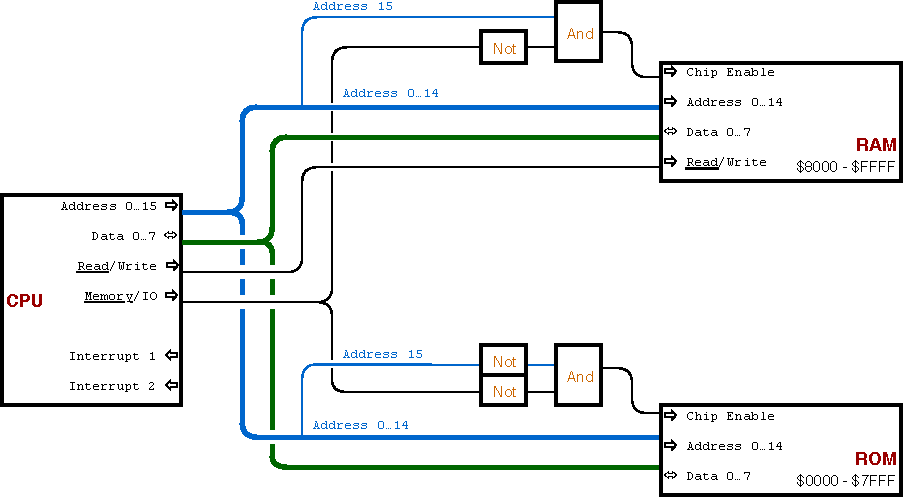
\includegraphics[width=\textwidth]{1-grundlagen/img/aufgabe-rechnerarchitektur-1}

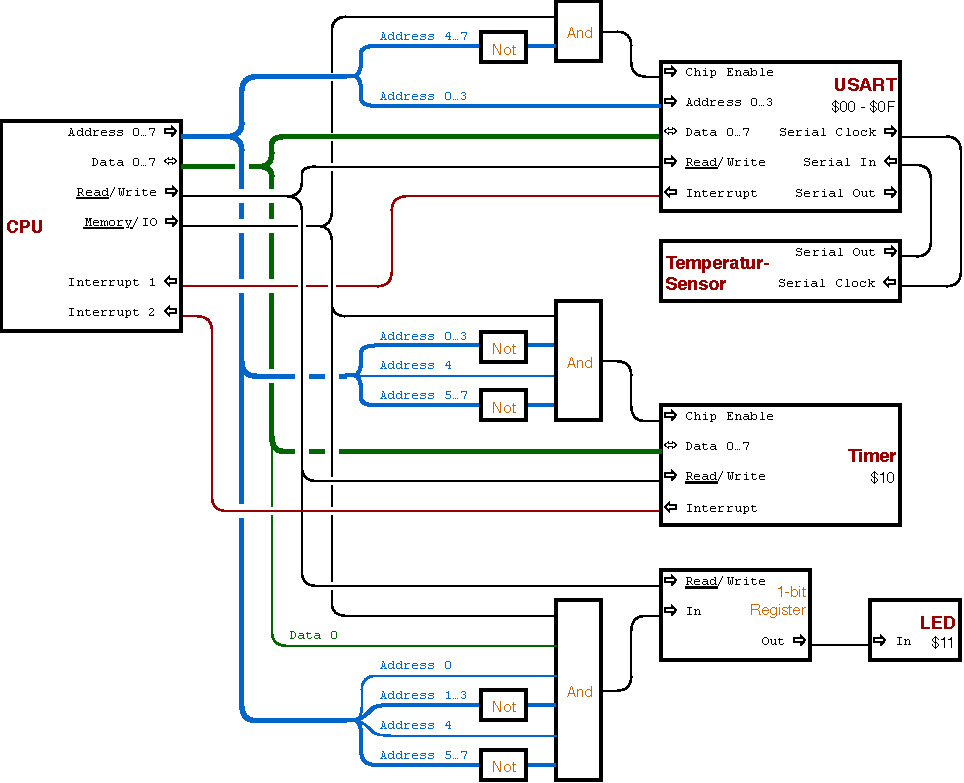
\includegraphics[width=\textwidth]{1-grundlagen/img/aufgabe-rechnerarchitektur-2}
\bigskip

Beantworten Sie die folgenden Fragen über das System:

\begin{enumerate}
    \item Welche Datenleitungen muss die CPU aktivieren, um einen Wert im
    Hauptspeicher abzulegen?

    \item Welche Datenleitungen muss die CPU stattdessen aktivieren, um den
    aktuellen Wert des Timers auszulesen? Welche Datenleitungen werden daraufhin
    vom Timerbaustein gesetzt, um den Wert zur Verfügung zu stellen?

    \item Handelt es bei dem I/O-Modell um \glqq{}Memory-Mappend I/O\grqq{}
    oder um \glqq{}Isolated I/O\grqq{} und woran lässt sich das erkennen?

    \item Wie funktioniert die Festlegung der Speicher- bzw. I/O-Adressen?
    Zeigen Sie, dass die im Blockdiagramm angegebenen Adressen
    (\texttt{\$8000} -- \texttt{\$FFFF} usw.) tatsächlich stimmen.
\end{enumerate}

\textbf{Hinweis:} Besitzt ein Bausteinen einen \texttt{Chip Enable}-Eingang,
muss dieser immer aktiv sein, um den Baustein anzusprechen. Andernfalls ignoriert
der Baustein sämtliche anderen Datenleitungen.

\clearpage

%-------------------------------------------------------------------------------
\aufgabe{Grundlagen der Assemblerprogrammierung}
%-------------------------------------------------------------------------------
In der folgenden Aufgabe soll ein kleines Programm für das oben gezeigte
System geschrieben werden. Da wir in Assembler programmieren, soll es sich
um ein ganz einfaches Programm handeln, das einfach in einer Endlosschleife
die aktuelle Temperatur ermittelt und die LED blinken lässt, sobald diese
10° Celsius unterschreitet. Hierfür müssen wir die I/O-Devices wie folgt
ansprechen:

\bigskip
{
    \setlength{\tabcolsep}{0pt}
    \small

    \begin{tabularx}{\textwidth}{X}
        \textbf{Serielle Schnittstelle:}
        \\
        Zunächst müssen wir in der I/O-Adresse \texttt{\$00} den ASCII-Code für den
        Buchstaben \texttt{R} (also den Wert \texttt{\$52}) und in der Adresse \texttt{\$01}
        die Anzahl der zu lesenden Bytes ablegen. Der USART-Baustein löst daraufhin einen
        Interrupt aus, sobald genügend Bytes empfangen wurden. Diese können wir dann
        aus den I/O-Adressen \texttt{\$00} bis \texttt{\$0F} auslesen.
        \\

        \smallskip
        \textbf{Temperatursensor:}
        \\
        Der Temperatursensor besitzt ein ganz simples Protokoll. Sobald wir die aktuelle
        Temperatur anfordern, erhalten wir zwei Bytes zurück. Das erste Byte beinhaltet
        einen Wert zwischen -150 und +150 und steht für die Zahl vor dem Komma. Das zweite
        Byte beinhaltet einen Wert zwischen 0 und 99 und steht für die beiden Zahlen
        nach dem Komma. Die Temperatur wird immer in Celsius zurückgegeben.
        \\

        \smallskip
        \textbf{Timer:}
        \\
        Der Timer hilft uns dabei, die LED blinken zu lassen, indem er in regelmäßigen
        Abständen einen Interrupt auslöst. Um ihn zu aktivieren müssen wir nur die Anzahl
        Millisekunden, die zwischen zwei Interrupts liegen soll, an die I/O-Adresse
        \texttt{\$10} schreiben. Die Zeitspanne muss mindestens 10 Millisekunden betragen.
        Andernfalls wird der Timer deaktiviert. Wird lesend auf den Timer zugegriffen,
        liefert er das eingestellte Intervall zurück.
        \\

        \smallskip
        \textbf{Leuchtdiode:}
        \\
        Die LED ist besonders genügsam. Schreiben wir eine Eins an die I/O-Adresse
        \texttt{\$11} fängt Sie an zu leuchten. Mit einer Null können wir sie wieder
        ausschalten.
        \\
    \end{tabularx}
}

\medskip
\teilaufgabe
Angenommen, wir könnten in einer beliebigen Programmiersprache einfach zwei
Unterprogramme definieren, die bei Eintreten der beiden Interrupts automatisch
aufgerufen werden. Und angenommen, wir könnten beliebige, globale und lokale
Variablen definieren und hätten folgende beiden Funktionen zur I/O-Kommunikation
zur Verfügung:

\bigskip
{
    \setlength{\tabcolsep}{0pt}
    \small

    \begin{tabularx}{\textwidth}{p{0.33\textwidth}X}
        \texttt{value = readIO(address)}
        &
        Liest den aktuellen Wert an der angegebenen I/O-Adresse.
        \\

        \texttt{writeIO(address, value)}
        &
        Schreibt einen Wert an die angegebene I/O-Adresse.
        \\
    \end{tabularx}
}

Wie könnte dann der Quellcode des Programms in Pseudocode aussehen? Sorgen Sie
dafür, dass am Anfang des Programms der Timer so eingestellt wird, dass er alle
250 Millisekunden feuert. Anschließend starten Sie eine Endlosschleife, in der
Sie den Temperatursensor auffordern, die aktuelle Temperatur zu messen und dann
abwarten, bis der Wert empfangen wurde. Erst dann dürfen Sie wieder eine neue
Temperatur anfordern, um eine bereits laufende Kommunikation mit dem Sensor nicht
zu unterbrechen! Liegt die Temperatur unter 10° Celsius, setzen Sie eine globale
Variable, anhand derer Sie erkennen können, dass die LED blinken soll. Die
Interruptroutine des Timers sagt Ihnen dabei, wann die LED ein- oder ausgeschaltet
werden soll.

\clearpage
\teilaufgabe
Um das eben erstellte Programm nun in Assembler ausprogrammieren zu können,
nehmen wir an, der Mikroprozessor wäre ein einfacher RISC-Prozessor mit einer
Load-Store-Architektur und daher auch nur sehr wenigen Assemblerbefehlen. Jeder
Wert, egal ob Speicheradresse oder symbolischer Wert zum Rechnen, muss daher
immer erst in eines von 16 Registern geschrieben werden, bevor damit irgend
etwas angefangen werden kann. Die Register sind hierfür einfach in Hex-Schreibweise
durchnummeriert:
\texttt{r0}, \texttt{r1}, \texttt{r2}, \texttt{r3}, \texttt{r4}, \texttt{r5},
\texttt{r6}, \texttt{r7}, \texttt{r8}, \texttt{r9}, \texttt{ra}, \texttt{rb},
\texttt{rc}, \texttt{rd}, \texttt{re}, \texttt{rf}

Folgende Befehle stellt uns der Prozessor zur Verfügung, wobei jedes Register
in den Beispielen durch jedes andere Register ausgetauscht werden kann. Ebenso
kann jeder Wert, der kein Befehl und kein Register ist, entweder dezimal (ohne
führendes Zeichen), hexadezimal (mit führendem Dollarzeichen) oder als Konstante
(mit führendem Rautezeichen) geschrieben werden.

\medskip
{
    \small

    \begin{longtable}{|p{\textwidth}|}
        \hline
        \verb|; Kommentar| \\
        Beschreibt einen Kommentar, der nicht übersetzt wird.
        \\

        \hline
        \verb|.const #name $cafe| \\
        Definiert eine Konstante mit dem Namen \verb|#name| und dem Wert \verb|$cafe|.
        Diese Anweisung erzeugt keinen Maschinencode, sondern dient dazu, häufig
        benötigte Werte oder Speicheradressen zu benennen.
        \\

        \hline
        \verb|wichtige_stelle:| \\
        Definiert eine Stelle im Quellcode, deren spätere ROM-Adresse mit
        \verb|#wichtige_stelle| ermittelt werden kann. Da es sich nur um eine
        Markierung im Quellcode handelt, erzeugt dies keinen Maschinencode.
        Die Syntax wird stattdessen benötigt, um eine Stelle zu markieren, an
        der das Programm nach einem Sprungbefehl weiterlaufen soll.
        \\

        %
        \hline
        \hline
        %

        \hline
        \verb|RGR r0, 32768| \\
        Schreibt die Zahl 32768 in das Register \texttt{r0}.
        \\

        \hline
        \verb|RGR r0, (32768)| \\
        Schreibt den Inhalt der Speicherzelle 32768 in das Register \texttt{r0}.
        \\

        \hline
        \verb|RGR r0, (r1)| \\
        Schreibt den Inhalt der durch \texttt{r1} angesprochenen Speicherzelle
        in das Register \texttt{r0}.
        \\

        \hline
        \verb|RGW r0, (32768)| \\
        Schreibt den Inhalt des Registers \texttt{r0} in die Speicherzelle 32768.
        \\

        \hline
        \verb|RGW r0, (r1)| \\
        Schreibt den Inhalt des Registers \texttt{r0} in die durch \texttt{r1}
        angesprochenen Speicherzelle
        \\

        \hline
        \verb|MOV r0, r1| \\
        Schreibt den Inhalt des Registers \texttt{r1} in das Register \texttt{r0}.
        \\

        %
        \hline
        \hline
        %

        \hline
        \verb|IOR r0, r1| \\
        List den Inhalt der in \texttt{r0} abgelegten I/O-Adresse in das Register
        \texttt{r1}.
        \\

        \hline
        \verb|IOW r0, r1| \\
        Schreibt den im Register \texttt{r1} übergebenen Wert in die I/O-Adresse
        in \texttt{r0}.
        \\

        %
        \hline
        \hline
        %

        \hline
        \verb|NOT r0| \\
        Kehrt den Inhalt des Register \texttt{r0} um, indem alle Bits negiert werden.
        \\

        \hline
        \verb|ADD r0, r1, r2| \\
        Addiert \texttt{r1} mit \texttt{r2} und speichert das Ergebnis in \texttt{r0}.
        \\

        \hline
        \verb|SUB r0, r1, r2| \\
        Subtrahiert \texttt{r2} von \texttt{r1} und speichert das Ergebnis in \texttt{r0}.
        \\

        \hline
        \verb|AND r0, r1, r2| \\
        Berechnet eine binäre Und-Verknüpfung zwischen \texttt{r1} und \texttt{r2}
        und legt das Ergebnis in \texttt{r0} ab.
        \\

        \hline
        \verb|OR r0, r1, r2| \\
        Berechnet eine binäre Oder-Verknüpfung zwischen \texttt{r1} und \texttt{r2}
        und legt das Ergebnis in \texttt{r0} ab.
        \\

        \hline
        \verb|XOR r0, r1, r2| \\
        Berechnet eine binäre Exklusiv-Oder-Verknüpfung zwischen \texttt{r1} und
        \texttt{r2} und legt das Ergebnis in \texttt{r0} ab.
        \\

        %
        \hline
        \hline
        %

        \hline
        \verb|JMP (r0)| \\
        Führt das Programm an der in \texttt{r0} übergebenen Speicherstelle fort.
        \\

        \hline
        \verb|JZR r0, (r1)| \\
        Führt das Programm bei \texttt{r1} übergebenen Speicherstelle fort,
        wenn der Wert in \texttt{r1} gleich Null ist.
        \\

        \hline
        \verb|JNZ r0, (r1)| \\
        Führt das Programm bei \texttt{r1} fort, wenn der Wert in \texttt{r1}
        ungleich Null ist.
        \\

        \hline
        \verb|JLT r0, (r1)| \\
        Führt das Programm bei \texttt{r1} fort, wenn der Wert in \texttt{r1}
        kleiner Null ist.
        \\

        \hline
        \verb|JLE r0, (r1)| \\
        Führt das Programm bei \texttt{r1} fort, wenn der Wert in \texttt{r1}
        kleiner oder gleich Null ist.
        \\

        \hline
        \verb|JGT r0, (r1)| \\
        Führt das Programm bei \texttt{r1} fort, wenn der Wert in \texttt{r1}
        größer Null ist.
        \\

        \hline
        \verb|JGE r0, (r1)| \\
        Führt das Programm bei \texttt{r1} fort, wenn der Wert in \texttt{r1}
        größer oder gleich Null ist.
        \\

        %
        \hline
        \hline
        %

        \hline
        \verb|RTI| \\
        Springt aus einer Interruptroutine wieder ins Hauptprogramm zurück.
        \\

        \hline
    \end{longtable}
}

% Mögliche Erweiterungen, für diese Aufgabe aber nicht relevant:
% Unterprogramme mit Rücksprungadresse, Stackbefehle, Signed/Unsigend Integer, …
%
%   » BRA (R0)
%   » JZR, JNZ, JLT, JLE, JGT, JGE  r0, (r1)
%   » RET
%   » PSH r0
%   » POP r0
%   » ADDU, SUBU r0, r1, r2

{
\footnotesize

\begin{verbatim}
  ; Konstanten und Variablen
  .const      #serial_address0      $00           ; I/O-Adresse: Serial 0
  .const      #serial_address1      $01           ; I/O-Adresse: Serial 1
  .const      #timer_address        $10           ; I/O-Adresse: Timer
  .const      #led_address          $11           ; I/O-Adresse: LED

  .const      #blink_intervall      250           ; Blink-Intervall der LED
  .const      #max_temperature      10            ; Temperatarugrenze

  .const      #read_temperature     $8000         ; Adresse der Variable #read_temperature
  .const      #current_temperature  $8001         ; Adresse der Variable #current_temperature
  .const      #blink_led            $8002         ; Adresse der Variable #blink_led
  .const      #led_status           $8003         ; Adresse der Variable #led_status

  ; Variablen initialisieren
  init_vars:
      RGR r0, 1                                   ; Den Wert 1 in die Variable
      RGW r0, (#read_temperature)                 ; #read_temperature schreiben

      RGR r0, 150                                 ; Den Wert 150 in die Variable
      RGW r0, (#current_temperature)              ; #current_temperature schreiben

      RGR r0, 0                                   ; Den Wert 0 in die Variablen
      RGW r0, (#blink_led)                        ; #blink_led und
      RGW r0, (#led_status)                       ; #led_status schreiben

  ; Timer initialisieren
  init_timer:
      RGR r0, #timer_address                      ; An die I/O-Adresse #timer_address
      RGR r1, #blink_intervall                    ; den Wert #blink_intervall
      IOW r0, r1                                  ; schreiben

  ; Endlosschleife des Hauptprogramms
  main:
·                                                 ; Nächste Befehle nur ausführen,
·                                                 ; wenn #read_temperature ungleich
·                                                 ; Null ist.

·                                                 ; An die I/O-Adresse #serial_address0
·                                                 ; das ASCII-Zeichen 'R' wie 'Read'
·                                                 ; schreiben

·                                                 ; An die I/O-Adresse #serial_address1
·                                                 ; den Wert 2 mit der Anzahl erwarteter
·                                                 ; Bytes schreiben

    main_check_temperature:
·                                                 ; Nächste Befehle nur ausführen,
·                                                 ; wenn der Wert der Variable
·                                                 ; #current_temperature kleiner als
·                                                 ; der Wert der Variable #max_temperature
·                                                 ; ist

·                                                 ; Den Wert 1 in die Variable
·                                                 ; #blink_led schreiben

    main_temparature_is_high:
·                                                 ; Den Wert 0 in die Variable
·                                                 ; #blink_led schreiben

    main_repeat:
·                                                 ; Zurück an den Anfang der
·                                                 ; Schleife springen

  ; Interruptroutine für den Temperatursensor
  isr1:
      RGR r0, #serial_address0                    ; Ersten vom Tempereratursensor
      IOR r0, r1                                  ; empfangenen Wert in der Variable
      RGW r1, (#current_temperature)              ; #current_temperature ablegen

      RGR r0, 1                                   ; Die Variable #read_temperature
      RGW r0, (#read_temperature)                 ; mit dem Wert 1 füllen

      RTI                                         ; Zurück zum Hauptprogramm

  ; Interruptroutine für den Timer
  isr2:
      RGR r1, 0                                   ; Neuer Wert der LED

      RGR r2, (#blink_led)                        ; Nächste Befehle nur ausführen,
      RGR r3, (#isr2_end)                         ; wenn die Variable #blink_led ungleich
      JZR r2, (r3)                                ; Null ist.

      RGR r1, (#led_status)                       ; Aktuellen Wert der Variablen #led_status
      NOT r1                                      ; umkehren

    isr2_end:
      RGR r0, #led_address                        ; An die I/O-Adresse #led_address
      IOW r0, r1                                  ; den neuen Wert der LED schreiben

      RTI                                         ; Zurück zum Hauptprogramm
\end{verbatim}
}



%===============================================================================
\clearpage
\LoesungHeader
%===============================================================================

%-------------------------------------------------------------------------------
\loesung{Eingebettete Systeme und IoT-Devices}
%-------------------------------------------------------------------------------
\teilaufgabe
Kriterien zur Definition von eingebetteter Systeme:
\DefinitionEmbedded{X}

\teilaufgabe
Kriterien zur Definition von IoT-Devices:
\DefinitionIoT{X}

\teilaufgabe
\glqq Deeply Embedded Systems\grqq{} im Vergleich zu anderen eingebetteten Systemen:

\begin{enumerate}
    \item Es handelt sich um kleinste Computersysteme mit in der Regel sehr
    geringer Komplexität und minimaler Systemausstattung.

    \setcounter{enumi}{2}   % Neuer Wert - 1
    \item Es handelt sich um besonders unauffällig arbeitende Computersysteme,
    deren Vorhandensein für den Benutzer oft nicht offensichtlich ist.
\end{enumerate}

\teilaufgabe
Themengebiete beim Entwurf einer IoT-Architektur (von unten nach oben):

\begin{enumerate}
    \item Elektronik
    \item Rechnerarchitektur
    \item Hardwareschnittstellen
    \item Hardwareplattformen
    \item Betriebssysteme der Devices
    \item Programmierung der Devices
    \item Kommunikationsprotokolle
    \item Backendkomponenten
    \item Benutzerseitige Komponenten
\end{enumerate}

\bigskip
\teilaufgabe
Anforderungen an die Software eines eingebetteten Systems:

\begin{longtable}{|p{0.44\textwidth} c p{0.45\textwidth}|}
    \hline
    Sparsame Ressourcennutzung
    & \textit{vs.} &
    \textcolor{gray}{\sout{Großzügige Zuteilung der Systemressourcen}}
    \\

    \hline
    \textcolor{gray}{\sout{Unterstützung üblicher Consumer-Hardware}}
    & \textit{vs.} &
    Unterstützung sehr spezialisierter Hardware
    \\

    \hline
    \textcolor{gray}{\sout{Geringe bis mittlere Nutzungsdauer am Tag}}
    & \textit{vs.} &
    Störungsfreier Betrieb über lange Zeit
    \\

    \hline
    Softwareupdates während dem Betrieb
    & \textit{vs.} &
    \textcolor{gray}{\sout{Updates in der Fachwerkstatt des Herstellers}}
    \\

    \hline
    \textcolor{gray}{\sout{Maximal flexible Systemarchitektur}}
    & \textit{vs.} &
    Vollständig deterministisches Systemverhalten
    \\

    \hline
    \textcolor{gray}{\sout{Nahezu unbegrenztes Multi-Tasking}}
    & \textit{vs.} &
    Feste Anzahl gleichzeitig laufender Tasks
    \\

    \hline
    \textcolor{gray}{\sout{Meist geringe Echtzeitanforderungen}}
    & \textit{vs.} &
    Erhöhte oder gar harte Echtzeitanforderungen
    \\

    \hline
    Ausschalten durch Trennen vom Strom
    & \textit{vs.} &
    \textcolor{gray}{\sout{Geordnetes Herunterfahren des Systems}}
    \\

    \hline
\end{longtable}

%-------------------------------------------------------------------------------
\loesung{Rechnerarchitekturen im Vergleich}
%-------------------------------------------------------------------------------
\teilaufgabe
Verschiedene Mikroprozessoren und Mikrocontroller im Vergleich:
\CPUVergleich{X}

\teilaufgabe
Fragen zum Blockdiagramm eines einfachen, eingebetteten Systems:

\bigskip
1. Um einen Wert im Hauptspeicher abzulegen, muss die CPU folgende Datenleitungen
aktivieren:

{
    \renewcommand{\arraystretch}{1.5}
    \small

    \begin{tabularx}{\textwidth}{p{0.2\textwidth}X}
        \texttt{Address 0…15}:
        &
        Adresse der gewünschten Speicherstelle.
        Die Adresse muss dabei größer oder gleich \texttt{\$8000} sein, so dass
        die oberste Adressleitung aktiv ist.
        \\

        \texttt{Data 0…7}:
        &
        Im Speicher abzulegender Wert.
        \\

        \texttt{\underline{Read}/Write}:
        &
        Muss aktiv sein (binär 1), damit ein Schreibzugriff erfolgt.
        \\

        \texttt{\underline{Memory}/IO}:
        &
        Muss inaktiv sein (binär 0), damit die Speicherbausteine
        angesprochen werden.
        \\
    \end{tabularx}
}

\medskip
2. Das Auslesen des Timers funktioniert prinzipiell auf die gleiceh Weise, nur
dass hier \texttt{\underline{Read}/Write} inaktiv und \texttt{\underline{Memory}/IO}
aktiv sein müssen. Die Adressleitungen \texttt{Address 0…15} müssen exakt die
Adresse \texttt{\$10} kodieren. Seinen Wert überträgt der Baustein durch Setzen
der entsprechenden Datenleitungen \texttt{Data 0…7}.

\medskip
3. Es handelt sich um \glqq{}Isolated I/O\grqq{}, da durch die
\texttt{\underline{Memory}/IO}-Leitung eindeutig unterschieden werden kann,
ob ein Speicherbaustein oder ein I/O-Device angesprochen werden soll. Im Gegensatz
\glqq{}Memory-Mappend I/O\grqq{} steht somit der volle Adressbereich für ROM und
RAM zur Verfügung, der Prozesser muss allerdings spezielle I/O-Befehle, die das
\texttt{\underline{Memory}/IO}-Signal aktivieren, zur Verfügung stellen. Computer
mit \glqq{}Memory-Mappend I/O\grqq{} besitzen ein solches Signal nicht, so dass
ein kleiner Teil des Speicherbereichs zum Ansprechen der I/O-Devices geopfert
werden muss. Der Zugriff erfolgt dann durch einfache Lese- und Schreibzugriffe
auf die von den Devices belegten Speicheradressen. Aus Sicht des Programmierers
legen sie ihre Daten sozusagen einfach im Hauptspeicher ab, auch wenn dies
technisch gesehen nicht stimmt.

\medskip
4. Zur Festlegung der Speicher- und I/O-Adressen werden einzelne Adressleitungen
mit \texttt{Not}- (negieren ein Signal und drehen es somit um) und \texttt{And}-Bausteinen
(geben nur dann ein aktives Signal aus, wenn sämtliche Eingänge aktiv sind)
verknüpft und anschließend auf \texttt{Chip\,Enable} des jeweiligen Bauteins
gelegt. Es handelt sich dabei um eine einfache Form der Adresskodierung, da
auf diese Weise sichergestellt wird, dass ein Baustein nur dann aktiv sein kann,
wenn eine für ihn bestimmte Adresse angesprochen wird. Anhand von RAM und ROM
lässt sich dies einfach zeigen: Hier wird die oberste Adressleitung \texttt{Adress\,15}
direkt mit \texttt{Chip\,Enable} des RAM-Bausteins verbunden (die \texttt{And}-Verknüpfung
dient hier nur dazu, I/O- und Speicherzugriffe zu unterscheiden). Somit muss das
oberste Adressbit immer gesetzt sein, um auf den Hauptspeicher zuzugreifen.
Binär können also nur die Adressen von \texttt{\%1000\,0000\,0000\,0000} bis
\texttt{\%1111\,1111\,1111\,1111} angesprochen werden, was Hexadezimal \texttt{\$8000}
bis \texttt{\$FFFF} entspricht. Beim ROM-Baustein ist \texttt{Chip\,Enable}
hingegen mit der negierten Version von \texttt{Adress\,15} belegt, so dass das
oberste Adressbit immer null sein muss. Die maximal zulässige Adresse im ROM
beträgt somit \texttt{\%0111\,1111\,1111\,1111} bzw. \texttt{\$7FFF}.

{
    \footnotesize
    Da allerdings weder ROM noch RAM das oberste Adressbit sehen, wird technisch
    gesehen in beiden Fällen immer eine Adresse zwischen \texttt{\$0000} bis \texttt{\$7FFF}
    angesprochen.
}

\clearpage

%-------------------------------------------------------------------------------
\loesung{Grundlagen der Assemblerprogrammierung}
%-------------------------------------------------------------------------------
\teilaufgabe
Pseudocode zum Auslesen der Temperatur und blinken einer LED, wenn es zu kalt ist:

{
\footnotesize

\begin{verbatim}
// Zunächst ein paar hilfreiche Konstanten und Variablen
const serialAddress0   = $00;
const serialAddress1   = $01;
const timerAddress     = $10;
const ledAddress       = $11;

const blinkIntervall   = 250;
const maxTemperature   = 10;

var readTemperature    = true;
var currentTemperature = 150;
var blinkLed           = false;
var ledStatus          = 0;

// Timer initialisieren
writeIO(timerAddress, blinkIntervall);

// Endlosschleife mit dem Hauptprogramm
while (true) {
    // Aktuelle Temperatur anfordern
    if (readTempertature) {
        readTemperature = false;
        writeIO(serialAddress0, 52);    // ASCII 'R'
        writeIO(serialAdress1, 2);      // 2-Bytes lesen
    }

    // LED blinken, wenn die Temperatur zu niedrig ist
    if (currentTemperature < maxTemperature) {
        blinkLed = true;
    } else {
        blinkLed = false;
    }
}

// Interruptroutine für den Temperatursensor
void handleSerialInterrupt() {
    currentTemperature = readIO(serialAddress0);
    readTemperature = true;
}

// Interruptroutine für den Timer
void handleTimerInterrupt() {
    if (blinkLed) {
        ledStatus = !ledStatus;
        writeIO(ledAddress, ledStatus);
    } else {
        writeIO(ledAddress, 0);
    }
}
\end{verbatim}
}

\clearpage
\teilaufgabe
Dasselbe Programm in Assembler für einen einfachen RISC-Prozessor mit
Load-Store-Architektur:

{
\footnotesize

\begin{verbatim}
; Konstanten und Variablen
.const      #serial_address0      $00           ; I/O-Adresse: Serial 0
.const      #serial_address1      $01           ; I/O-Adresse: Serial 1
.const      #timer_address        $10           ; I/O-Adresse: Timer
.const      #led_address          $11           ; I/O-Adresse: LED

.const      #blink_intervall      250           ; Blink-Intervall der LED
.const      #max_temperature      10            ; Temperatarugrenze

.const      #read_temperature     $8000         ; Adresse der Variable #read_temperature
.const      #current_temperature  $8001         ; Adresse der Variable #current_temperature
.const      #blink_led            $8002         ; Adresse der Variable #blink_led
.const      #led_status           $8003         ; Adresse der Variable #led_status

; Variablen initialisieren
init_vars:
    RGR r0, 1                                   ; Den Wert 1 in die Variable
    RGW r0, (#read_temperature)                 ; #read_temperature schreiben

    RGR r0, 150                                 ; Den Wert 150 in die Variable
    RGW r0, (#current_temperature)              ; #current_temperature schreiben

    RGR r0, 0                                   ; Den Wert 0 in die Variablen
    RGW r0, (#blink_led)                        ; #blink_led und
    RGW r0, (#led_status)                       ; #led_status schreiben

; Timer initialisieren
init_timer:
    RGR r0, #timer_address                      ; An die I/O-Adresse #timer_address
    RGR r1, #blink_intervall                    ; den Wert #blink_intervall
    IOW r0, r1                                  ; schreiben

; Endlosschleife des Hauptprogramms
main:
    RGR r0, #read_temperature                   ; Nächste Befehle nur ausführen,
    RGR r1, #main_check_temperature             ; wenn #read_temperature ungleich
    JZR r0, (r1)                                ; Null ist.

    RGR r0, #serial_address0                    ; An die I/O-Adresse #serial_address0
    RGR r1, 52                                  ; das ASCII-Zeichen 'R' wie 'Read'
    IOW r0, r1                                  ; schreiben

    RGR r0, #serial_address1                    ; An die I/O-Adresse #serial_address1
    RGR r1, 2                                   ; den Wert 2 mit der Anzahl erwarteter
    IOW r0, r1                                  ; Bytes schreiben

  main_check_temperature:
    RGR r1, (#current_temperature)              ; Nächste Befehle nur ausführen,
    RGR r2, (#max_temperature)                  ; wenn der Wert der Variable
    RGR r3, #main_temparature_is_high           ; #current_temperature kleiner als
    SUB r0, r1, r2                              ; der Wert der Variable #max_temperature
    JGE r0, (r3)                                ; ist

    RGR r0, 1                                   ; Den Wert 1 in die Variable
    RGW r0, (#blink_led)                        ; #blink_led schreiben

  main_temparature_is_high:
    RGR r0, 0                                   ; Den Wert 0 in die Variable
    RGW r0, (#blink_led)                        ; #blink_led schreiben

  main_repeat:
    RGR r0, #main                               ; Zurück an den Anfang der
    JMP (r0)                                    ; Schleife springen

; Interruptroutine für den Temperatursensor
isr1:
    RGR r0, #serial_address0                    ; Ersten vom Tempereratursensor
    IOR r0, r1                                  ; empfangenen Wert in der Variable
    RGW r1, (#current_temperature)              ; #current_temperature ablegen

    RGR r0, 1                                   ; Die Variable #read_temperature
    RGW r0, (#read_temperature)                 ; mit dem Wert 1 füllen

    RTI                                         ; Zurück zum Hauptprogramm

; Interruptroutine für den Timer
isr2:
    RGR r1, 0                                   ; Neuer Wert der LED

    RGR r2, (#blink_led)                        ; Nächste Befehle nur ausführen,
    RGR r3, (#isr2_end)                         ; wenn die Variable #blink_led ungleich
    JZR r2, (r3)                                ; Null ist.

    RGR r1, (#led_status)                       ; Aktuellen Wert der Variablen #led_status
    NOT r1                                      ; umkehren

  isr2_end:
    RGR r0, #led_address                        ; An die I/O-Adresse #led_address
    IOW r0, r1                                  ; den neuen Wert der LED schreiben

    RTI                                         ; Zurück zum Hauptprogramm
\end{verbatim}
}
